\documentclass[a4paper,12pt]{article}
\usepackage{setspace}
\usepackage[english]{babel}
\usepackage[utf8]{inputenc}
\usepackage{enumitem}
\usepackage{amsfonts}
\usepackage[margin=2.54cm]{geometry}
\usepackage{pdfpages}
\usepackage[utf8]{inputenc}
\usepackage[catalan]{babel}
\usepackage{graphicx,subcaption}
\usepackage{graphics}
\usepackage{lscape}
\usepackage{pdflscape}
\usepackage{float}
\usepackage{textcomp}
\usepackage{amsmath}
\usepackage{hyperref}
\usepackage{fancyvrb}
\usepackage{parskip}
\usepackage{changepage}
\usepackage{enumitem}
\usepackage{tcolorbox}
\usepackage[all]{hypcap}
\usepackage{xcolor}
\usepackage{listings}
\definecolor{green}{HTML}{228B22}
\definecolor{orange}{HTML}{FFA528}
\lstset{
    frame=tb, % draw a frame at the top and bottom of the code block
    tabsize=4, % tab space width
    showstringspaces=false, % don't mark spaces in strings
    numbers=left, % display line numbers on the left
    commentstyle=\color{green}, % comment color
    keywordstyle=\color{blue}, % keyword color
    stringstyle=\color{red}, % string color
    breaklines=true,
    numbers=left,
    xleftmargin=2em,
    framexleftmargin=1.5em,
    %postbreak=\mbox{\textcolor{red}{$\hookrightarrow$}\space},
}

\hypersetup{
    colorlinks,
    citecolor=black,
    filecolor=black,
    linkcolor=black,
    urlcolor=black
}
\title{
	\begin{center}
	\vspace{3cm}
	
\includegraphics[width=11cm, height=3cm]{images/logo_eps.png}
	\end{center}
	\begin{center}
	\line(1,0){340}
	\end{center}		
	SOFTWARE AND HARDWARE VALIDATION SYSTEMS\\
	\vspace{2mm}
	\Large Practical case 1: Verification of programs with Hoare logic and symbolic execution\\
	\line(1,0){340}
	\vspace{1.5cm}
	}

\author{Joel Aumedes Serrano - 48051307Y \\ Marc Cervera Rosell - 47980320C \vspace{1cm}}


\date{Academic course 2021 - 22\vspace{0.5cm} \\Bachelor's degree in computer engineering}
\onehalfspacing

\begin{document}
	\begin{titlepage}
		\maketitle
		\thispagestyle{empty}
	\end{titlepage}
	\cleardoublepage
	\newpage

\tableofcontents
\listoffigures
\thispagestyle{empty}

\newpage

\section{Exercise 1}
\begin{figure}[H]
    \centering
	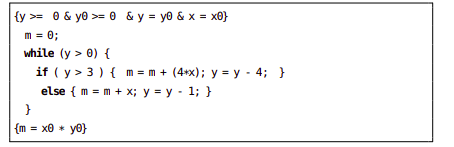
\includegraphics[scale = 0.75]{images/Screenshot from 2022-03-30 16-23-46.png}
	\caption{Exercise 1 code}
	\label{fig:code1}
\end{figure}
\justify{\textbf{\textit{Statement:}\\
Considering the breathtaking algorithm (see Figure~\ref{fig:code1}) for the multiplication of two integer numbers you must:\\
1. Obtain an appropiate invariant for the loop and explain it\\
2. Perform the verification of the partial correctness of the algorithm.}} \\

\subsection{Part 1}
\justify{Inv = \{\ x = x_{0} \ \& \ y $\geq$ 0 \ \& \ m = x_{0}*(y_{0} - y) \}\ }

\justify{\\ 
The value of 'x' never changes. \\
'y' starts $\geq$ 0, when it's '= 0', the loop ends.\\
At each step we add "x" and we substract 1 "y". When y = 0 $\rightarrow$ \mathcal{m = = x_{0} * y_{0}}.\\ }
\pagenumbering{arabic}
\newpage
\subsection{Part 2}
\justify{
\textit{Assignment rule:} \\
P = The same \\
$[$ m := 0 $]$ \\
while(y $>$ 0)\{ ... \} \\
Q = The same \\}

\justify{\textbf{Loop rules: \\}

\underline{Invariant initially valid (P $\rightarrow$ $\mathcal{U}$ (Inv)):} \\

\{\ y $\geq$ 0 \ \& \ y_{0} $\geq$ 0 \ \& \ y = y_{0} \ \& \ x = x_{0} \}\ \\
$\longrightarrow$ \\
\{\ x = x_{0} \ \& \ y $\geq$ 0 \ \& \ m = x_{0}*(y_{0} - y) \}\  \\ 
$[$ m := 0 $]$ \\ $\Downarrow$ \\
\{\ y $\geq$ 0 \ \& \ y_{0} $\geq$ 0 \ \& \ y = y_{0} \ \& \ x = x_{0} \}\ \\
$\longrightarrow$ \\
\{\ x = x_{0} \ \& \ y $\geq$ 0 \ \& \ 0 = x_{0}*(y_{0} - y) \}\ }
\newline

\begin{itemize}[label = {\checkmark}]
    \item x = $x_{0}$ is in P.
    \item y = $y_{0}$ is in P.
    \item ($y_{0}$ - y) = 0 because y = $y_{0}$ in P $\Rightarrow$ m = 0 = 0 * 0.
\end{itemize} \\

\newpage

\underline{Invariant preserved (\{ Inv \ \& \ b \} \[ \] $\rightarrow$ \{ Inv \}):} \\

$[$ m := 0 $]$ \\
\{\ $x = x_{0}$ \ \& \ y $\geq$ 0 \ \& \ m = $x_{0}$*$(y_{0}$ - y) \ y $>$ 0 \}\ \\

\begin{figure}[H]
    \centering
	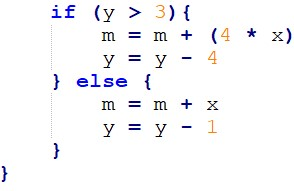
\includegraphics[scale = 1.0]{images/loop code.jpg}
	\caption{Loop code}
	\label{fig:loopCode}
\end{figure}

\textit{Quick remember:} \\
Inv = \{\ $x = x_{0}$ \ \& \ y $\geq$ 0 \ \& \ $m = x_{0}*(y_{0} - y)$ \}\

\subsubsection{Conditional rule $\rightarrow$ True side}
\{\ $x = x_{0}$ \ \& \ y $\geq$ 0 \ \& \ m = $x_{0}$*$(y_{0}$ - y) \ y $>$ 0 \ \& \ y $>$ 3 \}\ \\
$[$ m := 0 $||$ m := m + (4 * x) $||$ y := y - 4 $]$ (More than one assignment rule) \\
\{\ $x = x_{0}$ \ \& \ y $\geq$ 0 \ \& \ $m = x_{0}*(y_{0} - y)$ \}\ \\

\textit{Exit rule (P $\rightarrow$ $\mathcal{U}$ (Q)):} \\
\{\ $x = x_{0}$ \ \& \ y $\geq$ 0 \ \& \ m = $x_{0}$*$(y_{0}$ - y) \ y $>$ 0 \ \& \ y $>$ 3 \}\ \\
$\longrightarrow$ \\
\{ $x = x_{0}$ \ \& \ y - 4 $\geq$ 0 \ \& \ 0 + 4 * x = $x_{0} * (y_{0} - (y - 4))$ \}

\begin{itemize}[label = {\checkmark}]
    \item x = $x_{0}$ is in P.
    \item y = y $>$ 3 + y $\geq$ 4 $\rightarrow$ y- 4 $\geq$ 0.
    \item 4 * x = $x_{0}$ * $y_{0}$ - $x_{0}$ * y + 4 * x $\rightarrow$ 4 * x = $x_{0}$ * ($y_{0}$ - y) + 4 * x $\Rightarrow$ m = 0.
\end{itemize} \\
\newpage
\subsubsection{Conditional rule $\rightarrow$ False side}
\{\ $x = x_{0}$ \ \& \ y $\geq$ 0 \ \& \ m = $x_{0}$*$(y_{0}$ - y) \ y $>$ 0 \ \& \ !(y $>$ 3) \}\ \\
$[$ m := 0 $||$ m := m + x $||$ y := y - 1 $]$ (More than one assignment rule) \\

\textit{Exit rule (P $\rightarrow$ $\mathcal{U}$ (Q)):} \\
\{\ $x = x_{0}$ \ \& \ y $\geq$ 0 \ \& \ m = $x_{0}$*$(y_{0}$ - y) \ y $>$ 0 \ \& \ !(y $>$ 3) \}\ \\
$\longrightarrow$ \\
\{ $x = x_{0}$ \ \& $y - 1$ $\geq$ 0 \ \& \ 0 + x = $x = x_{0}$ * ($y_{0}$ - y + 1) \} \\
\begin{itemize}[label = {\checkmark}]
    \item x = $x_{0}$ is in P.
    \item y $\geq$ 0 is in P and y $\geq$ 1.
    \item 0 + x = $x = x_{0}$ * ($y_{0}$ - y + 1) $\rightarrow$ 0 + $x_{0}$ = $x_{0}$ * ($y_{0}$ - y) + $x_{0}$ $\Rightarrow$ m = 0.
\end{itemize} \\

\underline{Use case (\{ Inv \ \& \ !b \} \[ \] $\rightarrow$ \{ Q \}):} \\

\{\ $x = x_{0}$ \ \& \ y $\geq$ 0 \ \& \ m = $x_{0}$*$(y_{0}$ - y) \ !(y $>$ 0) \}\ \\
$[$ m := 0 $]$  (Assignment rule)\\
\{ m = $x_{0}$ * $y_{0}$ \} \\

\textit{Exit rule:}\\
\{\ $x = x_{0}$ \ \& \ y $\geq$ 0 \ \& \ m = $x_{0}$*$(y_{0}$ - y) \ !(y $>$ 0) \}\ \\
$\longrightarrow$ \\
$[$ m := 0 $]$ \\
\{ m = $x_{0}$ * $y_{0}$ \} \\
$\Downarrow$ \\
\{\ $x = x_{0}$ \ \& \ y $\geq$ 0 \ \& \ m = $x_{0}$*$(y_{0}$ - y) \ !(y $>$ 0) \}\ \\
$\longrightarrow$ \\
\{ m = $x_{0}$ * $y_{0}$ \} \\
\begin{itemize}[label = {\checkmark}]
    \item (!(y $>$ 0) \ \& \ y $\geq$ 0) $\rightarrow$ y = 0 $\Rightarrow$ m = $x_{0}$ * ($y_{0}$ - 0) = $x_{0}$ * $y_{0}$
\end{itemize} \\
\newpage

\section{Exercise 2}
\begin{figure}[H]
    \centering
	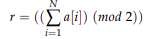
\includegraphics[scale = 1.0]{images/formula.png}
	\caption{Exercise 2 formula}
	\label{fig:formula1}
\end{figure}
\begin{figure}[H]
    \centering
	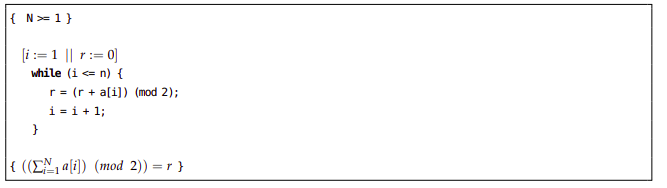
\includegraphics[scale = 0.70]{images/codi.png}
	\caption{Exercise 2 code}
	\label{fig:code2}
\end{figure}
\justify{\textbf{\textit{Statement:\\}
Verify the algorithm of the Figure~\ref{fig:code2} for computing the parity of the sum of the elements of an array a[N] with N \textbf{$\geq 0$} and storing it in the result variable r. You must:\\
1. Obtain an appropriate invariant for the loop and explain it.\\
2. Perform the verification of the partial correctness of the algorithm.}}



\end{document}
